\documentclass{article}
\usepackage{amssymb}
\usepackage{babel}
\usepackage{geometry}
\usepackage{amsmath}
\usepackage{amsthm}
\usepackage{framed}
\usepackage{pifont}
\usepackage{listings}
\usepackage{graphicx}
\usepackage{subcaption} 
\usepackage{subcaption} 
\usepackage{booktabs}
\usepackage{multirow}
\usepackage{xcolor}
\usepackage{array}
\usepackage{hyperref}
\usepackage{booktabs}
\usepackage{tabularx}


\definecolor{codegray}{gray}{0.9}
\lstset{
    backgroundcolor=\color{codegray},
    basicstyle=\ttfamily\small,
    breaklines=true,
    frame=single
}


\def\ra{\rightarrow}
\def\oo{\infty}
\def\l/{\backslash}
\def\0{\emptyset}
\def\b{\,\,\,}
\def\mm{{\mu^*}}
\def\hm{\mathcal{H}^s}
\def\vm{\nu^*}
\def\cui{\bigcup_{i=1}^\infty}
\def\cai{\bigcap_{i=1}^\infty}
\def\cuj{\bigcup_{j=1}^\infty}
\def\caj{\bigcap_{j=1}^\infty}
\def\sumj{\sum_{j=1}^\infty}
\def\sumi{\sum_{i=1}^\infty}
\def\sumn{\sum_{n=1}^\infty}
\def\px{\mathcal{P}_X}
\def\s{\mathcal{S}}
\def\a{\mathcal{A}}
\def\bs{\mathcal{B}}
\def\lm{\mathcal{L}}
\def\R{\mathbb{R}}
\def\E{\mathbb{E}}
\def\Z{\mathbb{Z}}
\def\m{\mathcal{M}}
\def\rr{\Rightarrow}
\def\tf{$\Rightarrow$}
\def\f{\mathcal{F}}
\def\limn{\lim_{n \rightarrow \infty}}
\def\st{\text{s.t.}}
\def\sums{ \sum_{x \in \s}}

%Ricky Def
\def\baru{\bar{\mu}}
\def\Mbaru{\mathfrak{M}_{\baru}}


\title{COMP4211 PA2 Report} 
\author{Name: Ruiming Min; SID: 20827430; ITSC: rmin}
\date{\today}

\begin{document}

    
\maketitle

\section*{Notice:}
\textbf{Since features of the} \LaTeX \textbf{ file, most of the images and tables are not shown under the discirbation. You can find them by index. Also, you can click the index to jump to the corresponding figure or table.}

\section*{5 Datasets and Data Loaders}

\subsection*{5.3 Dataloader Implementation}

\subsubsection*{[Q1]}
Number of images in COCO dataset: 3557.
Number of images in WikiArt dataset: 7492.

\subsubsection*{[Q2]}
Number of images in PACS train dataset: 1641.
Number of images in PACS test dataset: 2723.

\newpage

\section*{6 Style Transfer}

\subsection*{6.2 Model}

\subsubsection*{[Q3]}
Since after encoding, the image is represented as a 3D tensor and its 2D shape is much smaller than the original image. 
Therefore, in the decoder, we need the upsampling-re-construct the image-its original size.

\subsubsection*{[Q4]}
For each layer, we have the trainable parameters as follows:
\begin{itemize}
    \item Conv2d: $(k \times k \times c_{in} + 1) \times c_{out}$
    \item Pooling and Upsampling: 0
\end{itemize}

Therefore, the total number of trainable parameters is 2332511.

\subsubsection*{[Q5]}
Since the we need encoder-encode the image and mine the features, but if we only use the encoder, we cannot re-construct the image. 
Therefore, we need the decoder-re-construct the image.

\subsubsection*{[Q6]}
Since in this model, we do not only need the style match our target style, but also need the content-be preserved.
Therefore, we need-use the content loss and style loss-balance the style transfer.

\subsection*{6.4 Training the Style Transfer model}

\subsubsection*{[Q7]}

After 60 epochs, total loss is 12832.387, content loss is 7974.505, and style loss is 4857.882.

\subsection*{6.5 Inference}

\subsubsection*{[Q8]}

From the figure \ref{fig:part1_inference}, we can see the style transfer examples.
In these comparisons, we can see that the generated images represented the content of the content images very well expect the words in them.
For the style, the generated images are very similar-the style images in color and painting techniques.
However, if the style is very different from the content, the generated images may not be very good (e.g.: picture l).
Moreover, the generated images have some strange textures in some areas, which may be caused by the imbalance of the style data set, i.e., there are too many paintings in the training set.

% input images in a 3*2 grid
\begin{figure}[h!]
    \centering
    % First row of subfigures
    \begin{minipage}{\textwidth}
        \centering
        \begin{subfigure}{0.25\textwidth}
            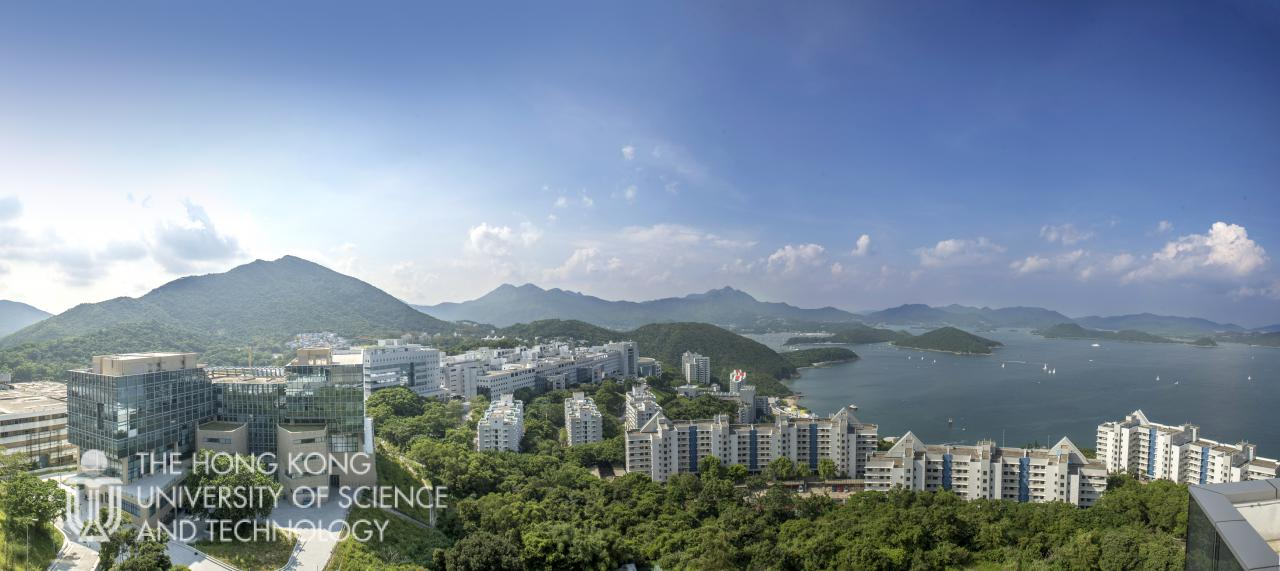
\includegraphics[width=\textwidth]{./data_set/HKUST/1.jpg}
            \caption{Content Image}
        \end{subfigure}
        \hfill % This command adds space between the subfigures
        \begin{subfigure}{0.25\textwidth}
            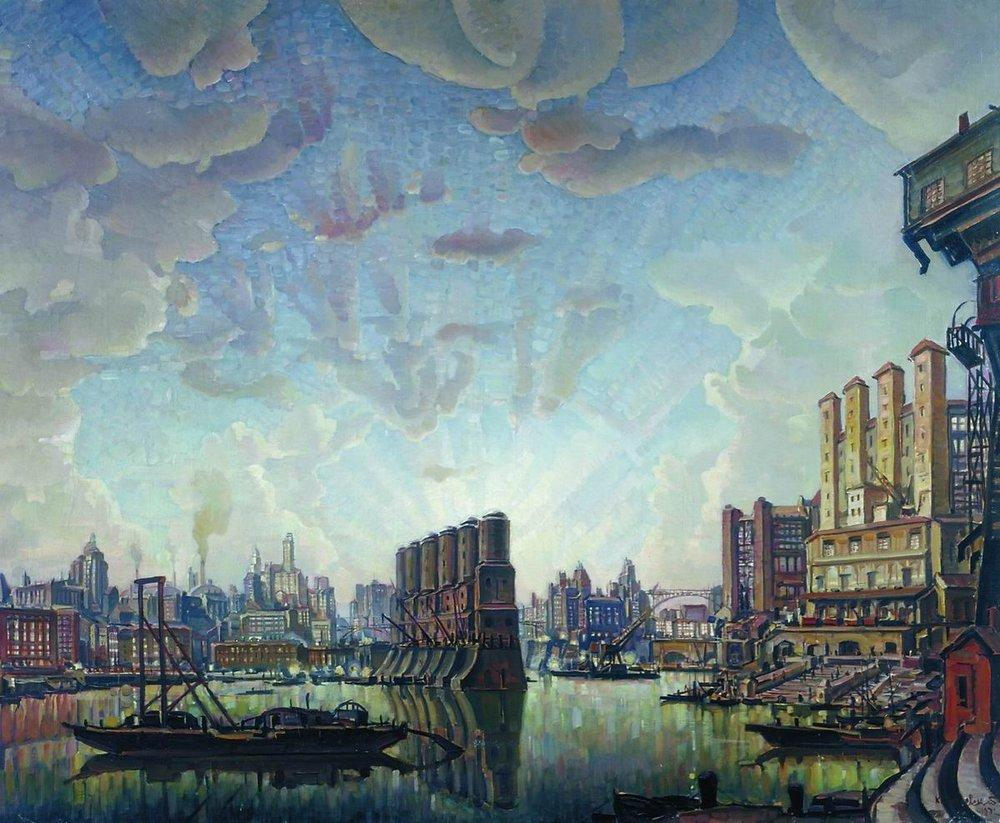
\includegraphics[width=\textwidth]{./wikiart/Symbolism/konstantin-bogaevsky_port-of-imaginary-city-1932.jpg}
            \caption{Style Image}
        \end{subfigure}
        \hfill % This command adds space between the subfigures
        \begin{subfigure}{0.25\textwidth}
            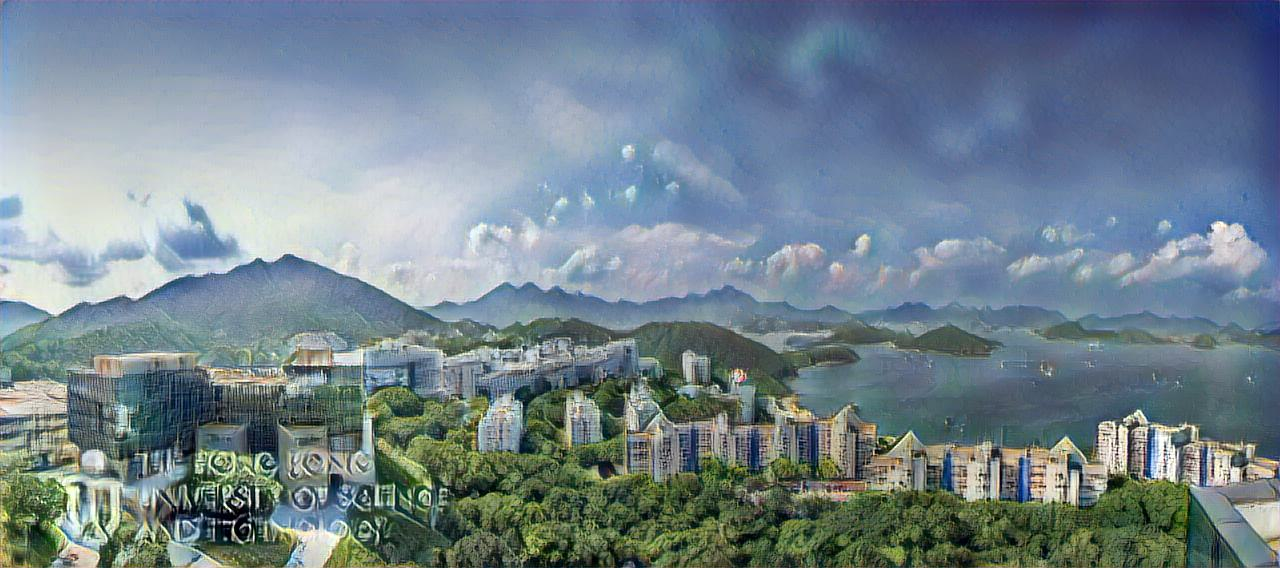
\includegraphics[width=\textwidth]{./part1_inference/output_1_konstantin-bogaevsky_port-of-imaginary-city-1932.jpg}
            \caption{Generated Image}
        \end{subfigure}
    \end{minipage}
    
    \vspace{0.1cm} % This command adds vertical space between the rows
    
    % Second row of subfigures
    \begin{minipage}{\textwidth}
        \centering
        \begin{subfigure}{0.25\textwidth}
            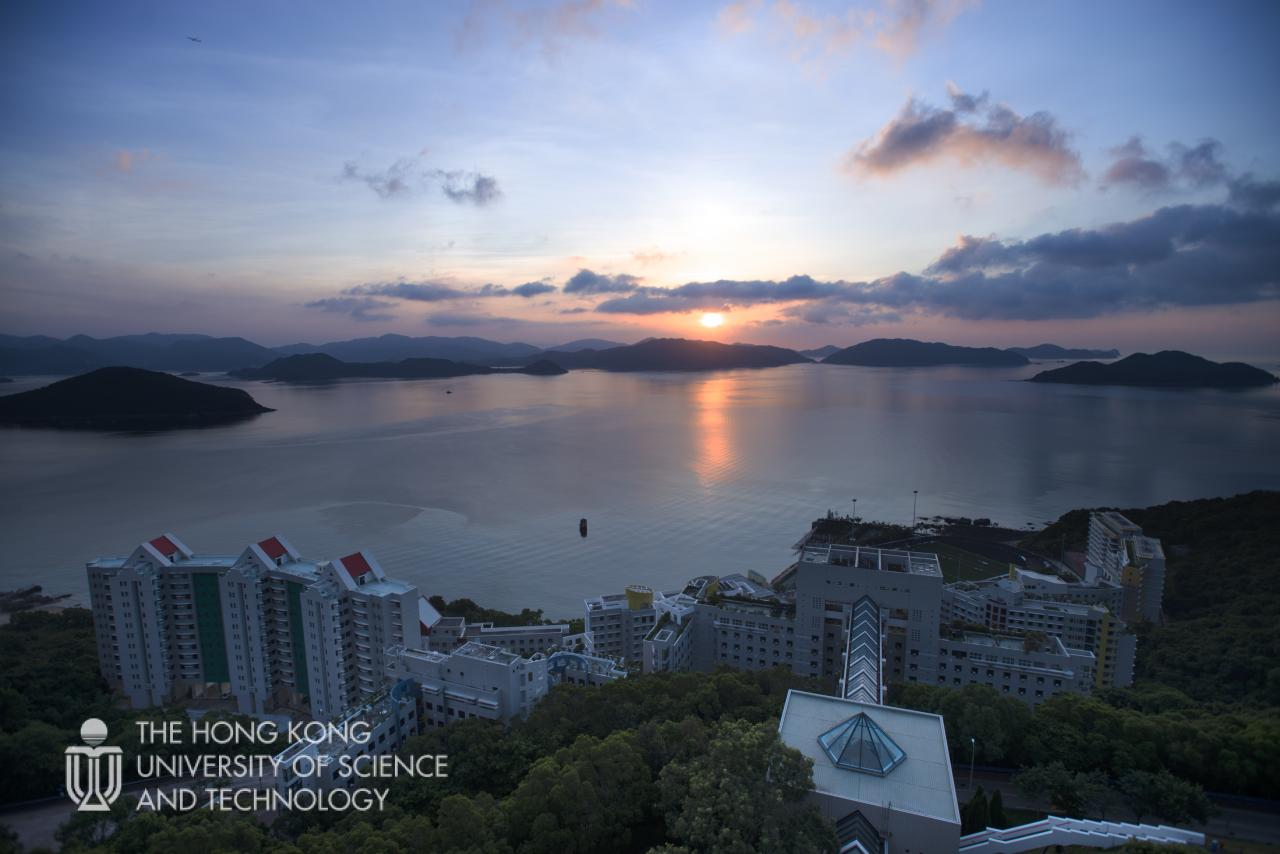
\includegraphics[width=\textwidth]{./data_set/HKUST/2.jpg}
            \caption{Content Image}
        \end{subfigure}
        \hfill % This command adds space between the subfigures
        \begin{subfigure}{0.25\textwidth}
            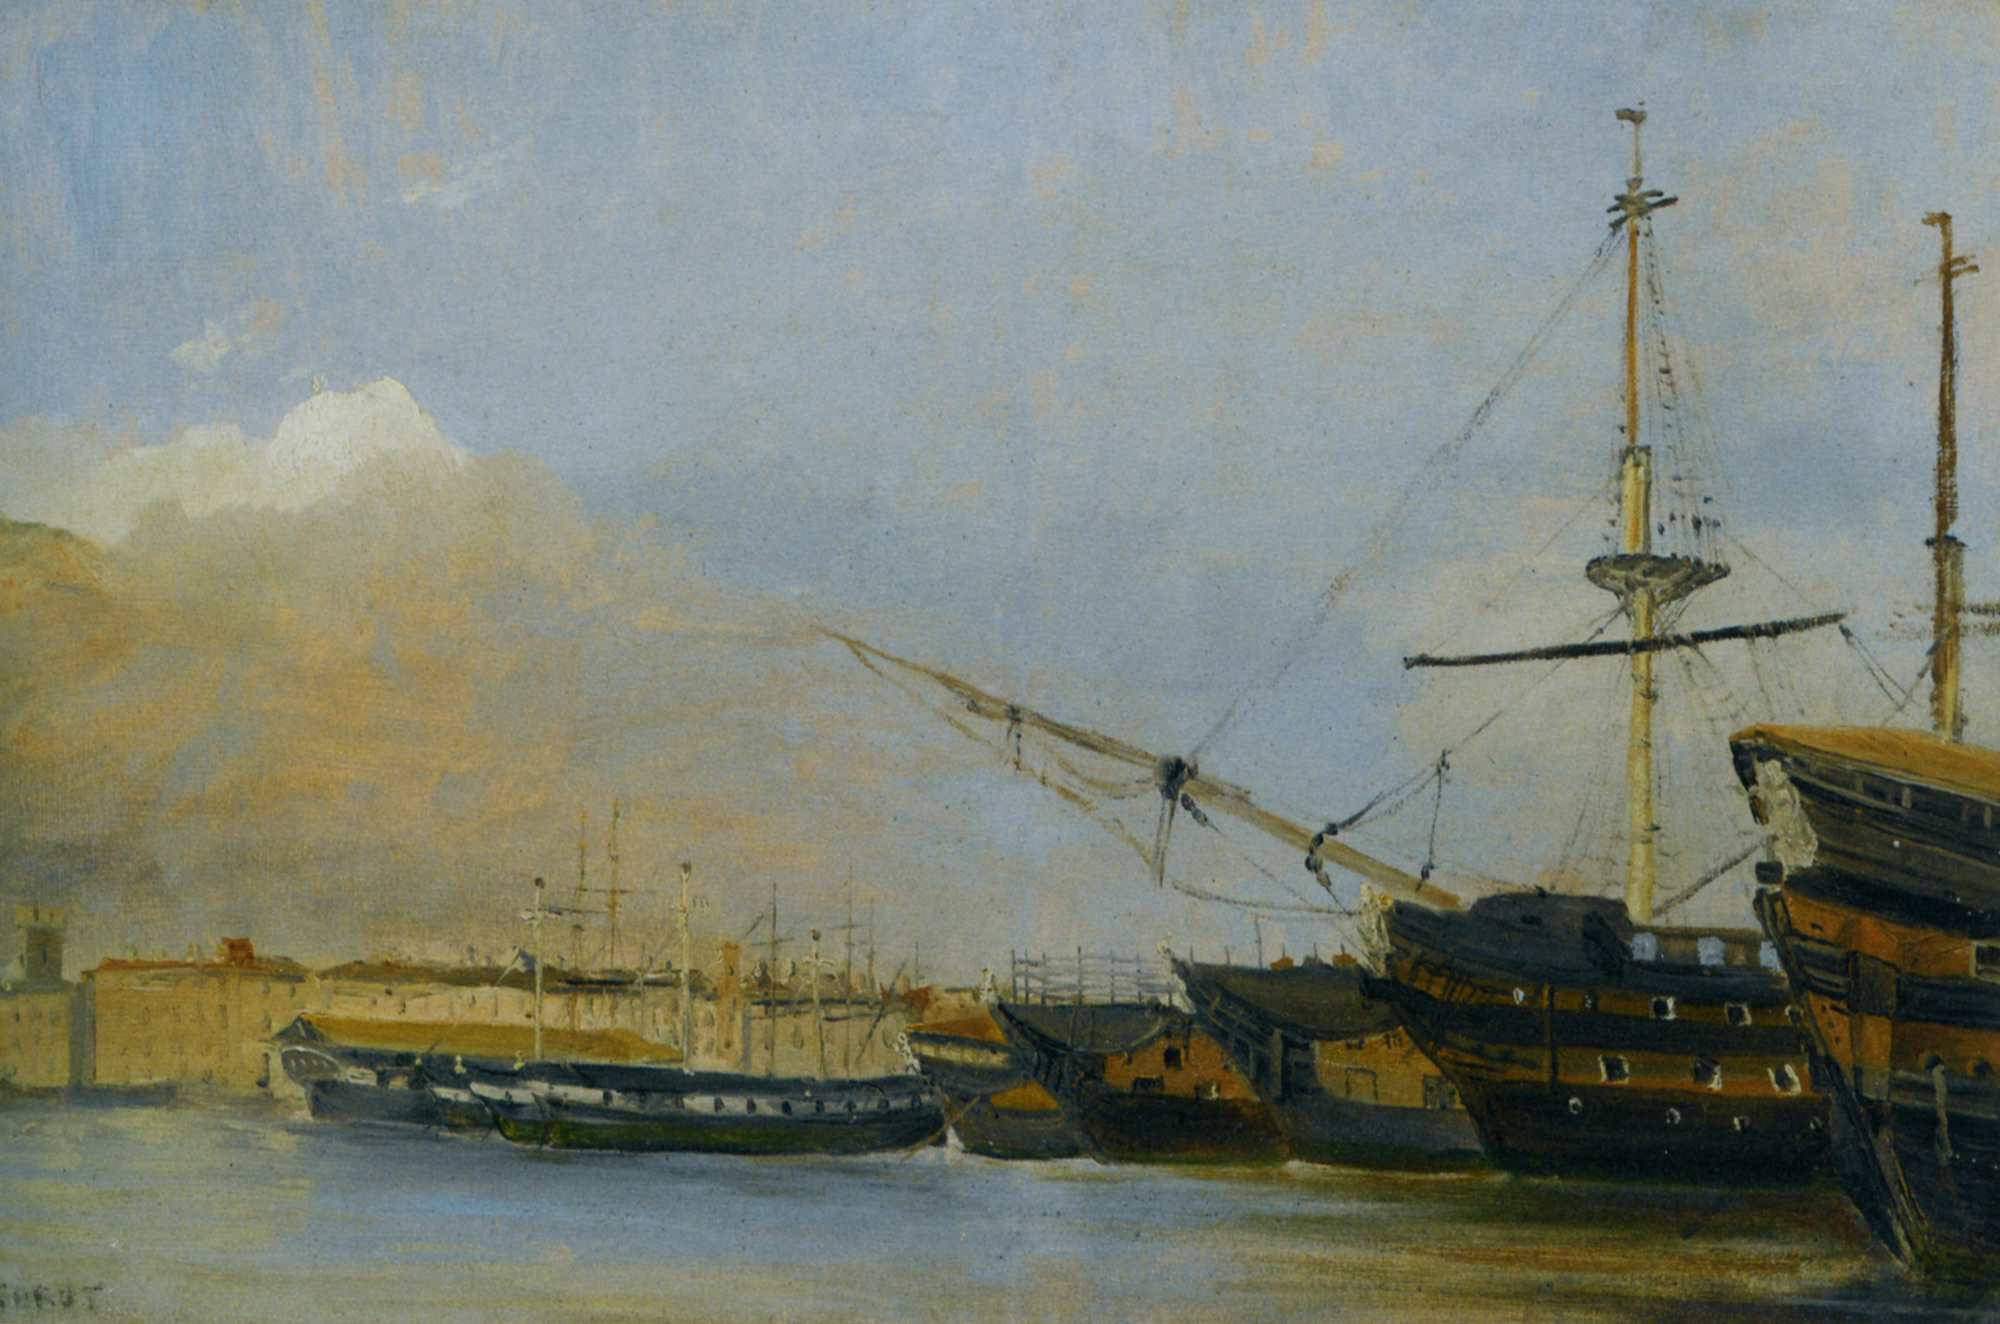
\includegraphics[width=\textwidth]{./wikiart/Realism/camille-corot_toulon-battleships-dismantled.jpg}
            \caption{Style Image}
        \end{subfigure}
        \hfill % This command adds space between the subfigures
        \begin{subfigure}{0.25\textwidth}
            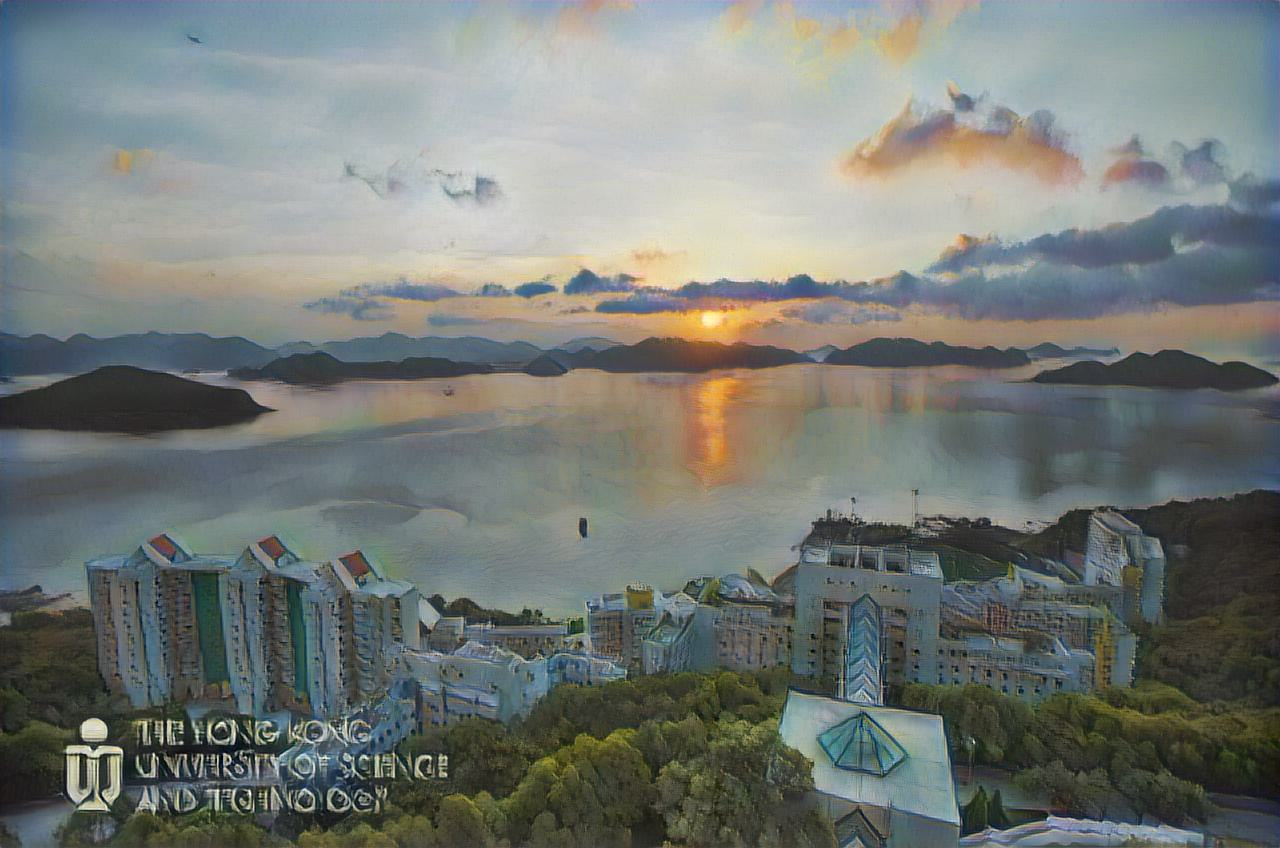
\includegraphics[width=\textwidth]{./part1_inference/output_2_camille-corot_toulon-battleships-dismantled.jpg}
            \caption{Generated Image}
        \end{subfigure}
    \end{minipage}
    
    \vspace{0.1cm}

    \begin{minipage}{\textwidth}
        \centering
        \begin{subfigure}{0.25\textwidth}
            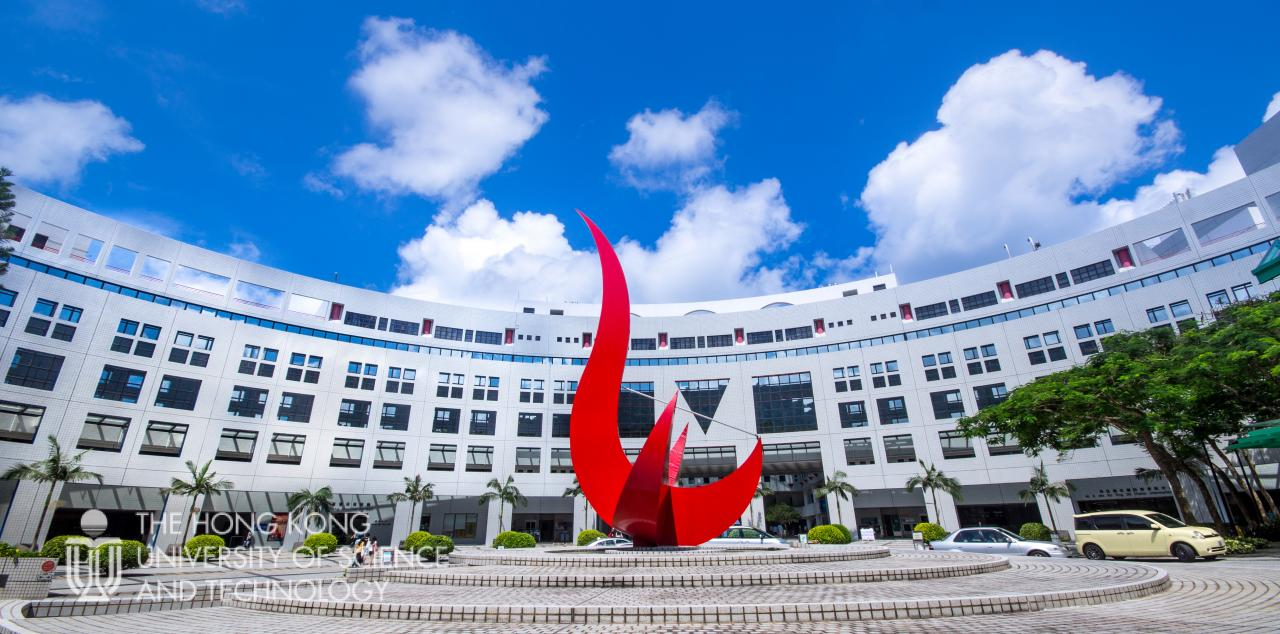
\includegraphics[width=\textwidth]{./data_set/HKUST/3.jpg}
            \caption{Content Image}
        \end{subfigure}
        \hfill % This command adds space between the subfigures
        \begin{subfigure}{0.25\textwidth}
            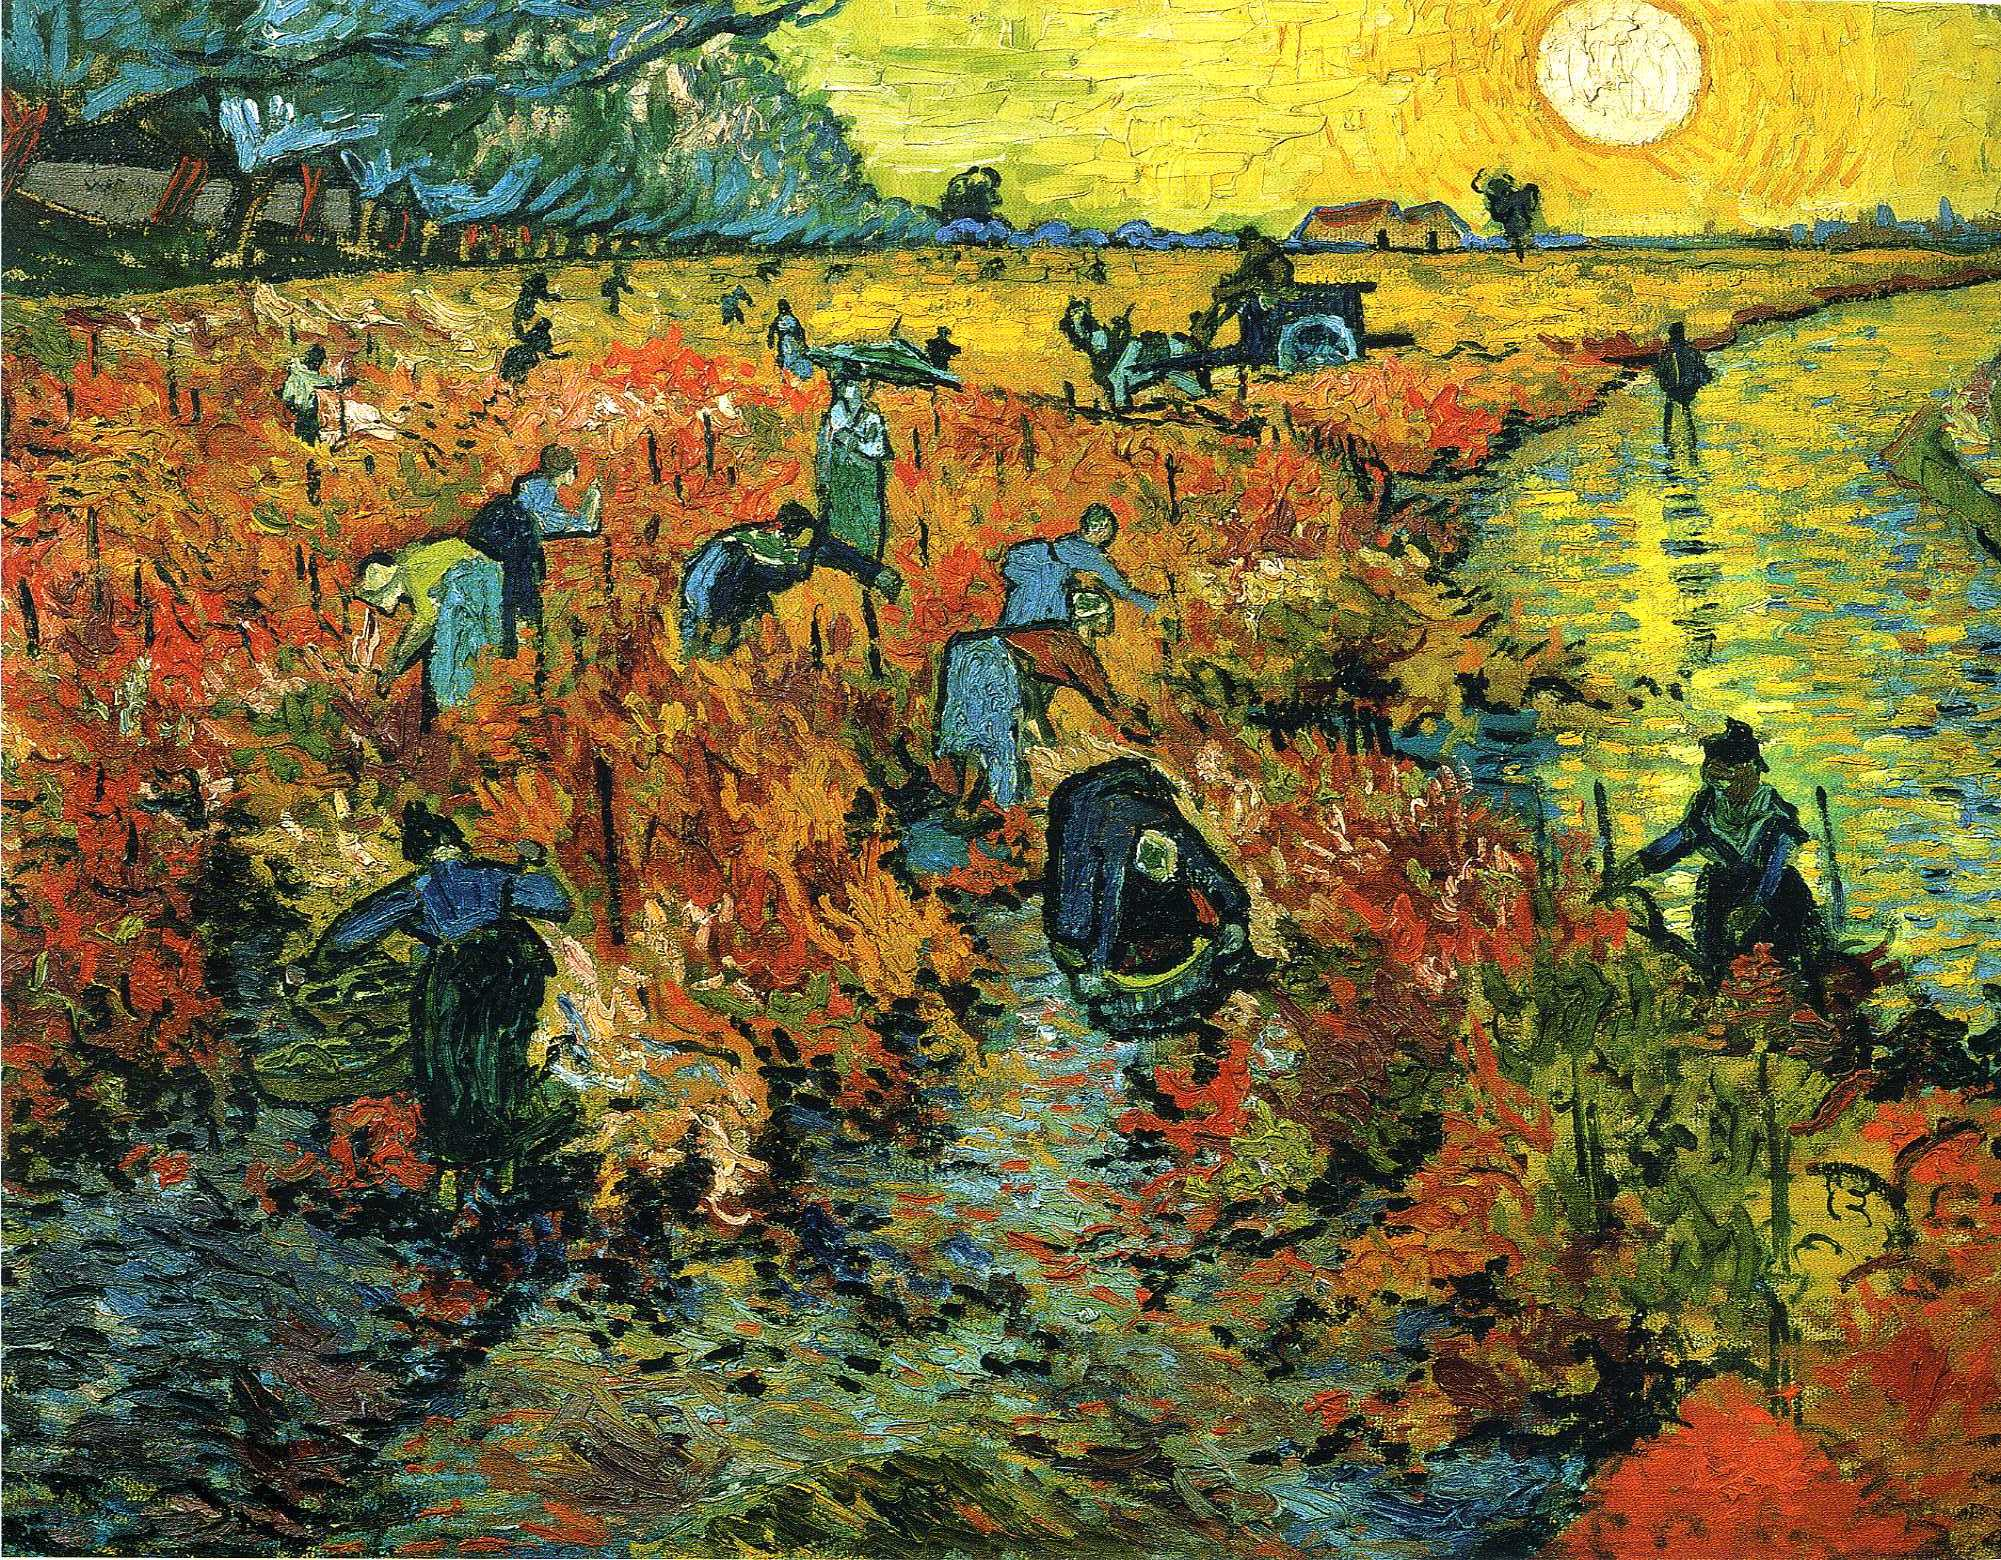
\includegraphics[width=\textwidth]{./wikiart/Post_Impressionism/vincent-van-gogh_red-vineyards-at-arles-1888.jpg}
            \caption{Style Image}
        \end{subfigure}
        \hfill % This command adds space between the subfigures
        \begin{subfigure}{0.25\textwidth}
            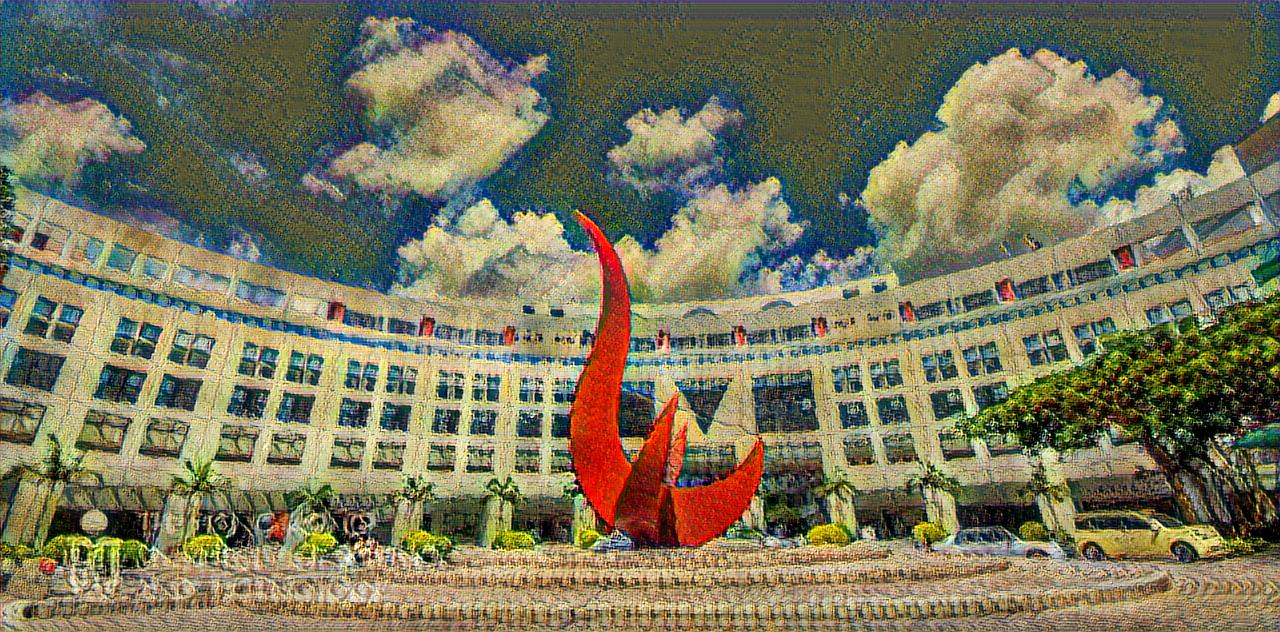
\includegraphics[width=\textwidth]{./part1_inference/output_3_vincent-van-gogh_red-vineyards-at-arles-1888.jpg}
            \caption{Generated Image}
        \end{subfigure}
    \end{minipage}
    
    \vspace{0.1cm}

    \begin{minipage}{\textwidth}
        \centering
        \begin{subfigure}{0.25\textwidth}
            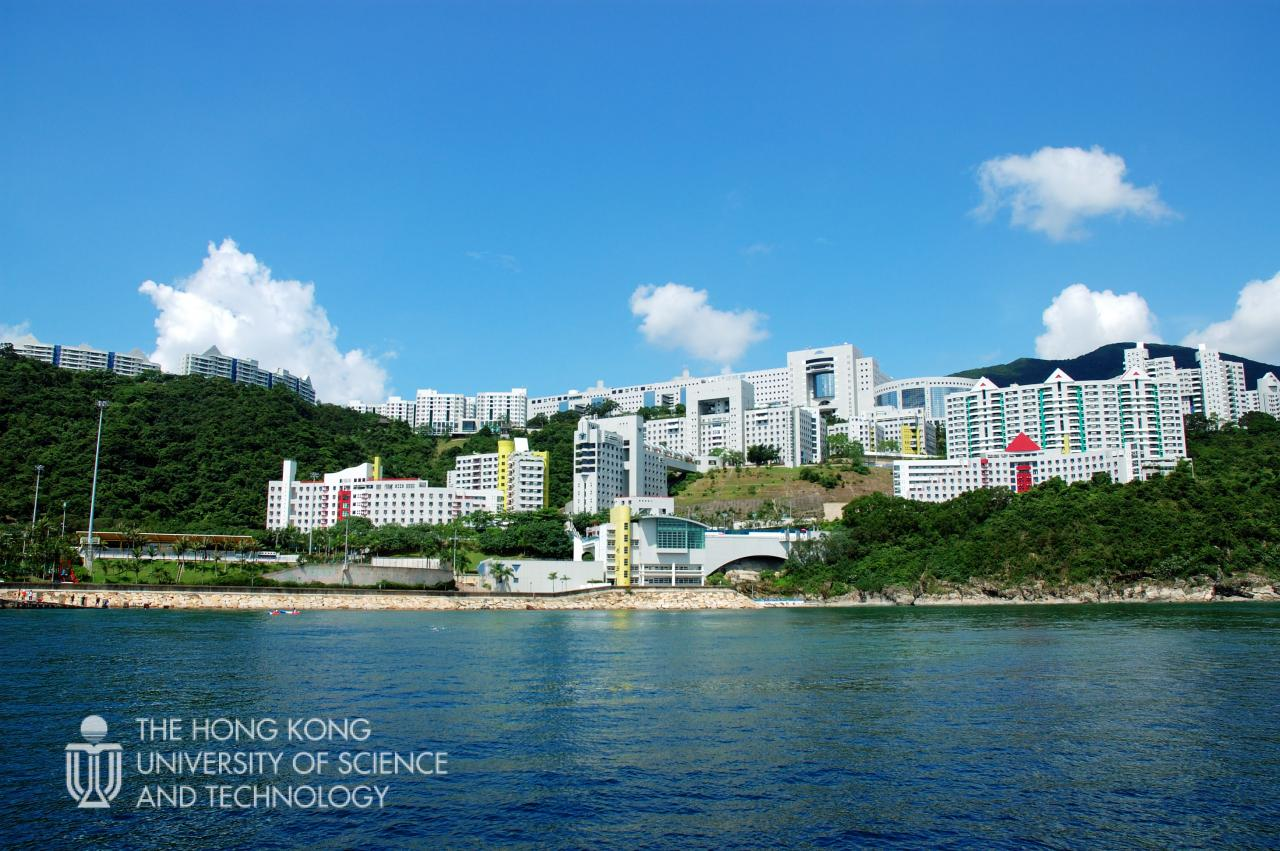
\includegraphics[width=\textwidth]{./data_set/HKUST/6.jpeg}
            \caption{Content Image}
        \end{subfigure}
        \hfill % This command adds space between the subfigures
        \begin{subfigure}{0.25\textwidth}
            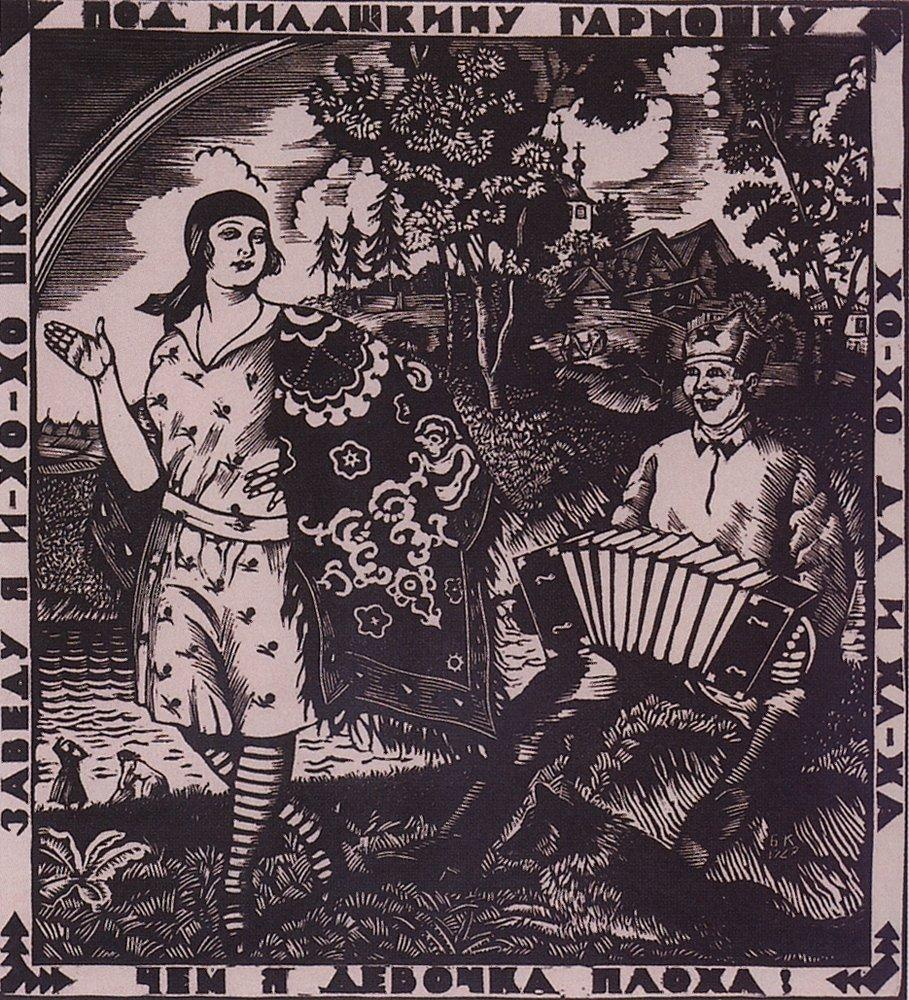
\includegraphics[width=\textwidth]{./wikiart/Art_Nouveau_Modern/boris-kustodiev_under-honey-s-harmonica-1927.jpg}
            \caption{Style Image}
        \end{subfigure}
        \hfill % This command adds space between the subfigures
        \begin{subfigure}{0.25\textwidth}
            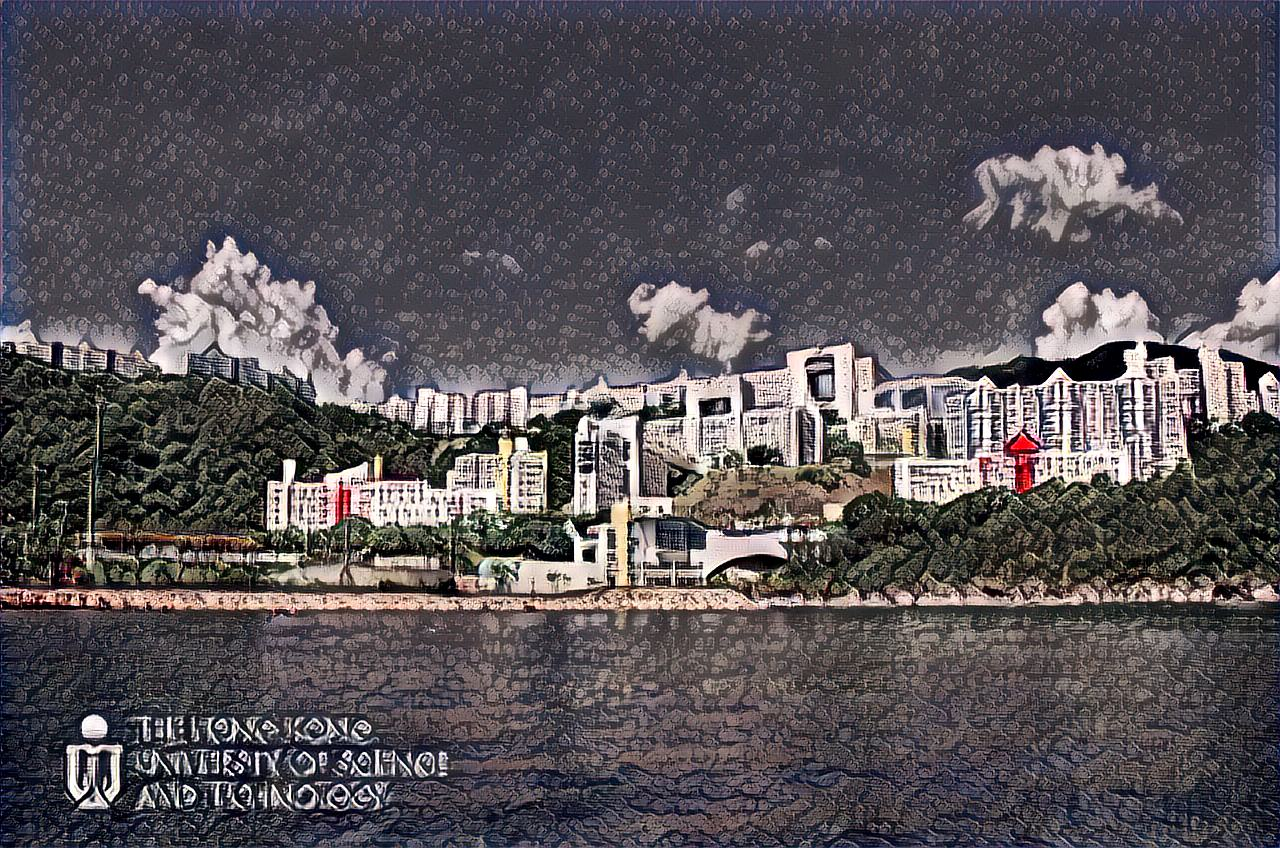
\includegraphics[width=\textwidth]{./part1_inference/output_6_boris-kustodiev_under-honey-s-harmonica-1927.jpg}
            \caption{Generated Image}
        \end{subfigure}
    \end{minipage}
    
    \vspace{0.1cm}

    \begin{minipage}{\textwidth}
        \centering
        \begin{subfigure}{0.25\textwidth}
            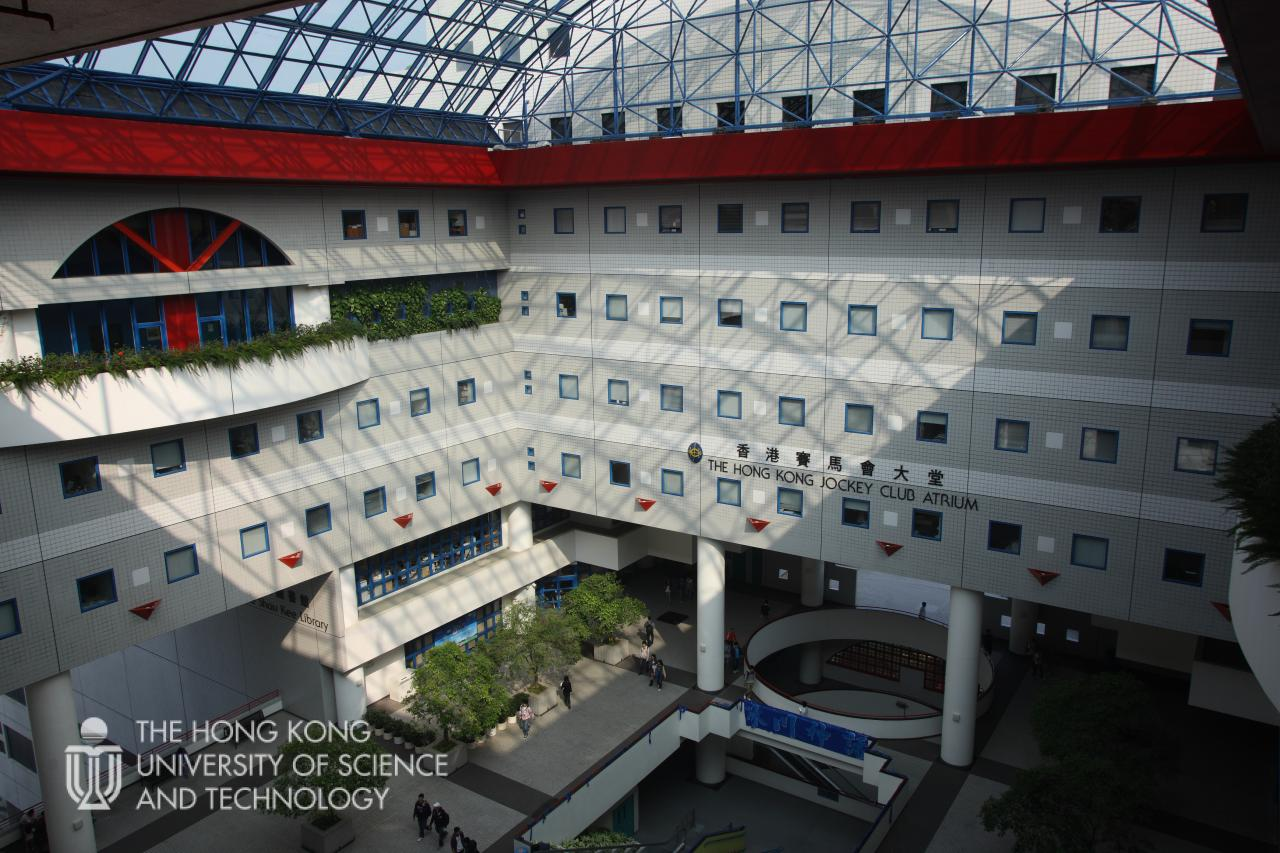
\includegraphics[width=\textwidth]{./data_set/HKUST/14.jpeg}
            \caption{Content Image}
        \end{subfigure}
        \hfill % This command adds space between the subfigures
        \begin{subfigure}{0.25\textwidth}
            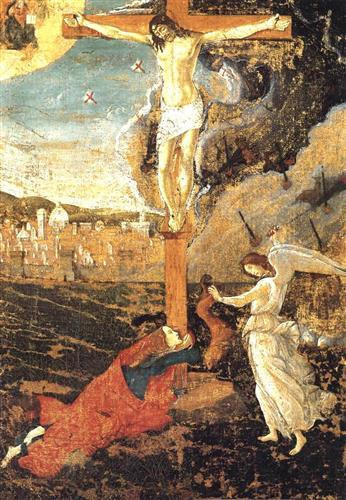
\includegraphics[width=\textwidth]{./wikiart/Early_Renaissance/sandro-botticelli_crucifixion(1).jpg}
            \caption{Style Image}
        \end{subfigure}
        \hfill % This command adds space between the subfigures
        \begin{subfigure}{0.25\textwidth}
            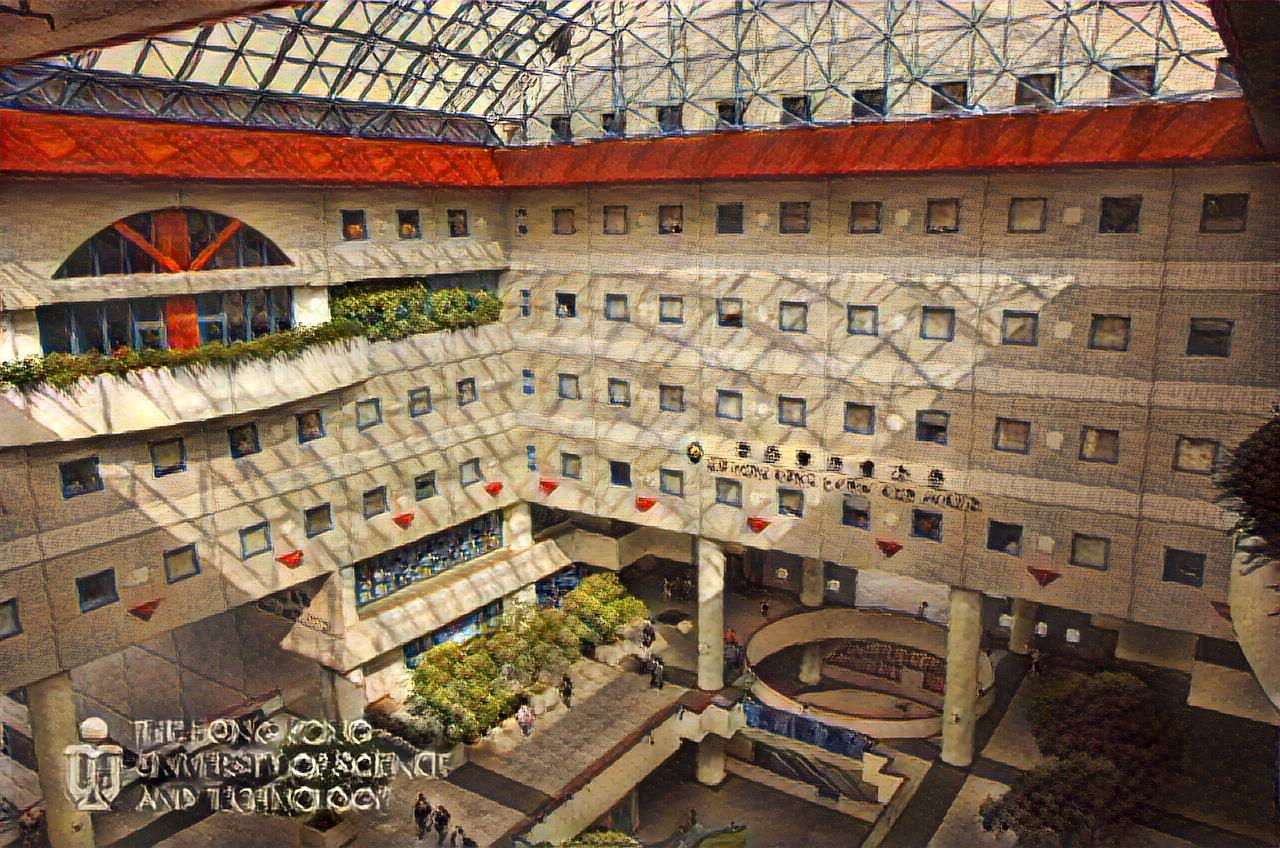
\includegraphics[width=\textwidth]{./part1_inference/output_14_sandro-botticelli_crucifixion(1).jpg}
            \caption{Generated Image}
        \end{subfigure}
    \end{minipage}    
    
    \caption{Example of Style Transfer}
    \label{fig:part1_inference}
\end{figure}

\newpage

\section*{7 Classification Task}

\subsection*{7.2 Analyzing the Dataset}

\subsubsection*{[Q9]}

From the figure \ref{fig:class_distribution}, and the output of the code (table \ref{tab:dataset_distribution}), 
we can see that the training and testing dataset distributions are very similar expect house and guitar.
The ratios of training samples of house and guitar are less than the testing samples.
And the number of training samples of each class is a half of the testing samples.

Moreover, the highest different between training and testing samples is that there are many type-animal pair only were shown a little in the training dataset but shown a lot in the testing dataset.

\begin{table}[ht]
    \centering
    \caption{Combined Training and Test Data Counts}
    \label{tab:dataset_distribution}
    \begin{tabular}{llrr}
        \toprule
        \multicolumn{2}{c}{Category} & \multicolumn{1}{c}{Training Count} & \multicolumn{1}{c}{Test Count} \\
        \cmidrule(lr){1-2} \cmidrule(lr){3-3} \cmidrule(lr){4-4}
        Label Type & Label Animal & Count & Count \\
        \midrule
        art\_painting & dog & 13 & 119 \\
        art\_painting & elephant & 13 & 89 \\
        art\_painting & giraffe & 231 & 110 \\
        art\_painting & guitar & 10 & 82 \\
        art\_painting & horse & 180 & 90 \\
        art\_painting & house & 11 & 110 \\
        art\_painting & person & 11 & 96 \\
        cartoon & dog & 10 & 95 \\
        cartoon & elephant & 13 & 83 \\
        cartoon & giraffe & 12 & 109 \\
        cartoon & guitar & 121 & 82 \\
        cartoon & horse & 11 & 81 \\
        cartoon & house & 12 & 101 \\
        cartoon & person & 12 & 95 \\
        photo & dog & 10 & 81 \\
        photo & elephant & 13 & 83 \\
        photo & giraffe & 12 & 102 \\
        photo & guitar & 10 & 81 \\
        photo & horse & 11 & 103 \\
        photo & house & 215 & 95 \\
        photo & person & 211 & 110 \\
        sketch & dog & 229 & 112 \\
        sketch & elephant & 217 & 115 \\
        sketch & giraffe & 10 & 104 \\
        sketch & guitar & 9 & 95 \\
        sketch & horse & 8 & 108 \\
        sketch & house & 13 & 80 \\
        sketch & person & 13 & 112 \\
        \bottomrule
    \end{tabular}
    \end{table}

% input images for training and testing
\begin{figure}[h!]
    \centering
% First row of subfigures
    \begin{subfigure}{0.45\textwidth}
        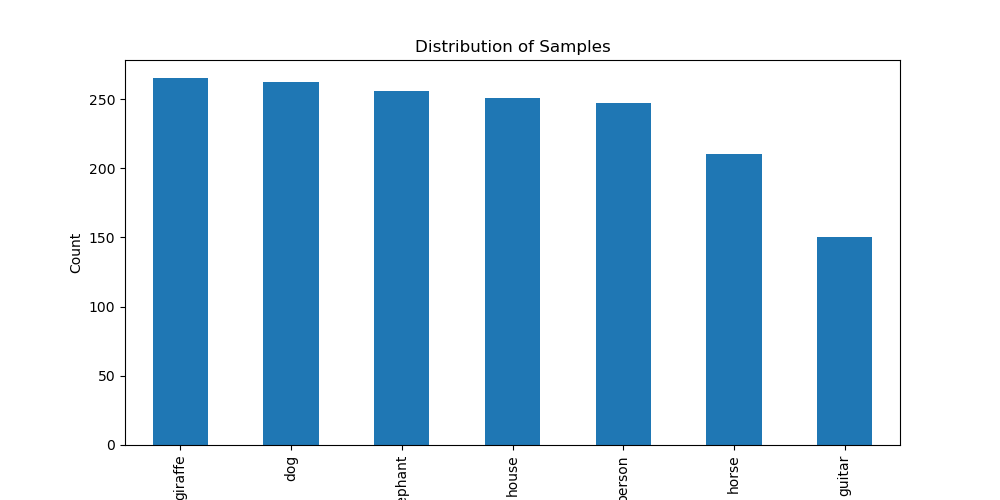
\includegraphics[width=\textwidth]{./pic/class_distribution_1641.png}
        \caption{Train Image}
    \end{subfigure}
    \hfill % This command adds space between the subfigures
    \begin{subfigure}{0.45\textwidth}
        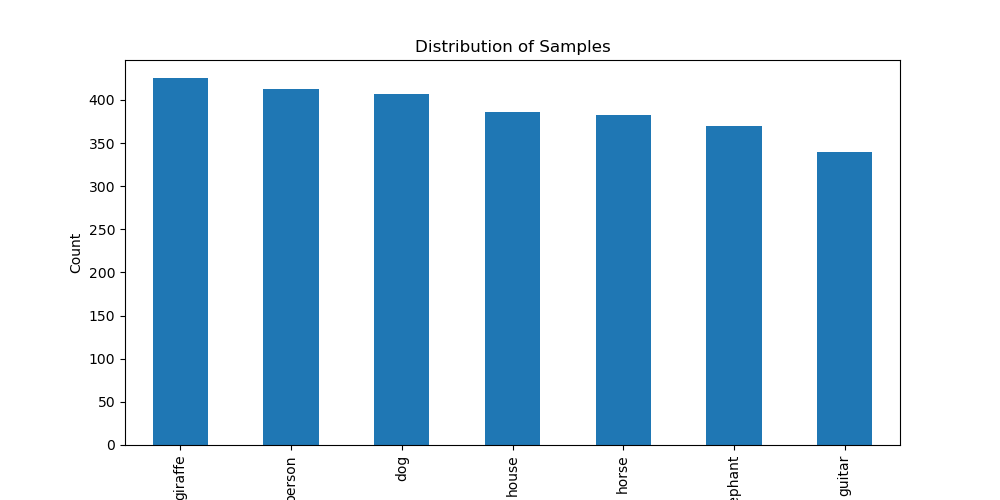
\includegraphics[width=\textwidth]{./pic/class_distribution_2723.png}
        \caption{Test Image}
    \end{subfigure}
    \caption{Class Distribution}
    \label{fig:class_distribution}
\end{figure}


\subsubsection*{[Q10]}
Since horse and guitar have less training samples, the model may not be able-learn the features of these two classes very well.
Therefore, the model may not be able-classify the horse and guitar very well.

Also, since the imbalance of training samples, the model may not be able-classify some type-animal pairs very well. For example, since the number of art\_painting-dog is small in the training dataset, the model may not be able-classify the art\_painting-dog very well.


\subsection*{7.3 Model Implementation}

\subsubsection*{[Q11]}

For each layer, we have the trainable parameters as follows:
\begin{itemize}
    \item Dense Layer: $(n_{in} + 1) \times n_{out}$
    \item Pooling: 0
\end{itemize}

Therefore, the total number of trainable parameters is 2103303.


\subsection*{7.4 Training the Classification model}

\subsubsection*{[Q12]}

After 160 epochs, the cross-entropy loss is 0.856, the detailed loss summary is shown in the table \ref{tab:cross_entropy_loss}.
\begin{table}[ht]
    \centering
    \caption{Cross-Entropy Loss Summary Every 10 Epochs}
    \begin{tabular}{cc}
    \toprule
    Epoch & Cross-Entropy Loss \\
    \midrule
    10  & 1.505 \\
    20  & 1.409 \\
    30  & 1.306 \\
    40  & 1.256 \\
    50  & 1.214 \\
    60  & 1.164 \\
    70  & 1.132 \\
    80  & 1.091 \\
    90  & 1.047 \\
    100 & 1.023 \\
    110 & 0.968 \\
    120 & 0.955 \\
    130 & 0.911 \\
    140 & 0.888 \\
    150 & 0.856 \\
    160 & 0.755 \\
    \bottomrule
    \end{tabular}
    \label{tab:cross_entropy_loss}
\end{table}


\subsection*{7.5 Testing Routine}

\subsubsection*{[Q13]}

The accuracy of training dataset is 0.690, and the accuracy of testing dataset is 0.250.

The confusion matrix is shown in the table \ref{tab:confusion_matrix_train} and table \ref{tab:confusion_matrix_test}.

Also, I visualize the confusion matrix in the figure \ref{fig:confusion_matrix_train} and figure \ref{fig:confusion_matrix_test}.

\begin{center}
    \textbf{Confusion Matrix for Train}
    
    \begin{tabular}{c|ccccccc}
    \toprule
    & \multicolumn{7}{c}{Predicted Labels} \\
    \cmidrule(lr){2-8}
    True Labels & dog & elephant & giraffe & guitar & horse & house & person \\
    \midrule
    dog & 240 & 0 & 8 & 2 & 5 & 4 & 2 \\
    elephant & 216 & 25 & 5 & 1 & 5 & 1 & 2 \\
    giraffe & 10 & 3 & 187 & 27 & 13 & 12 & 11 \\
    guitar & 17 & 3 & 13 & 108 & 2 & 2 & 1 \\
    horse & 10 & 0 & 29 & 5 & 137 & 10 & 15 \\
    house & 13 & 0 & 9 & 1 & 4 & 216 & 2 \\
    person & 13 & 0 & 9 & 4 & 8 & 6 & 204 \\
    \bottomrule
    \end{tabular}
    \captionof{table}{Confusion matrix for the training dataset.}
    \label{tab:confusion_matrix_train}
\end{center}

    
    
\begin{center}
    \textbf{Confusion Matrix for Test}
    
    \begin{tabular}{c|ccccccc}
    \toprule
    & \multicolumn{7}{c}{Predicted Labels} \\
    \cmidrule(lr){2-8}
    True Labels & dog & elephant & giraffe & guitar & horse & house & person \\
    \midrule
    dog & 122 & 2 & 76 & 49 & 54 & 61 & 43 \\
    elephant & 127 & 21 & 51 & 44 & 48 & 44 & 34 \\
    giraffe & 104 & 4 & 118 & 92 & 29 & 54 & 23 \\
    guitar & 103 & 6 & 44 & 81 & 47 & 20 & 39 \\
    horse & 110 & 3 & 66 & 37 & 87 & 48 & 30 \\
    house & 86 & 7 & 74 & 23 & 31 & 142 & 23 \\
    person & 123 & 7 & 72 & 27 & 48 & 26 & 110 \\
    \bottomrule
    \end{tabular}
    \captionof{table}{Confusion matrix for the testing dataset.}
    \label{tab:confusion_matrix_test}
\end{center}


% import confusion matrix
\begin{figure}[h!]
    \centering
    % First row of subfigures
    \begin{subfigure}{0.45\textwidth}
        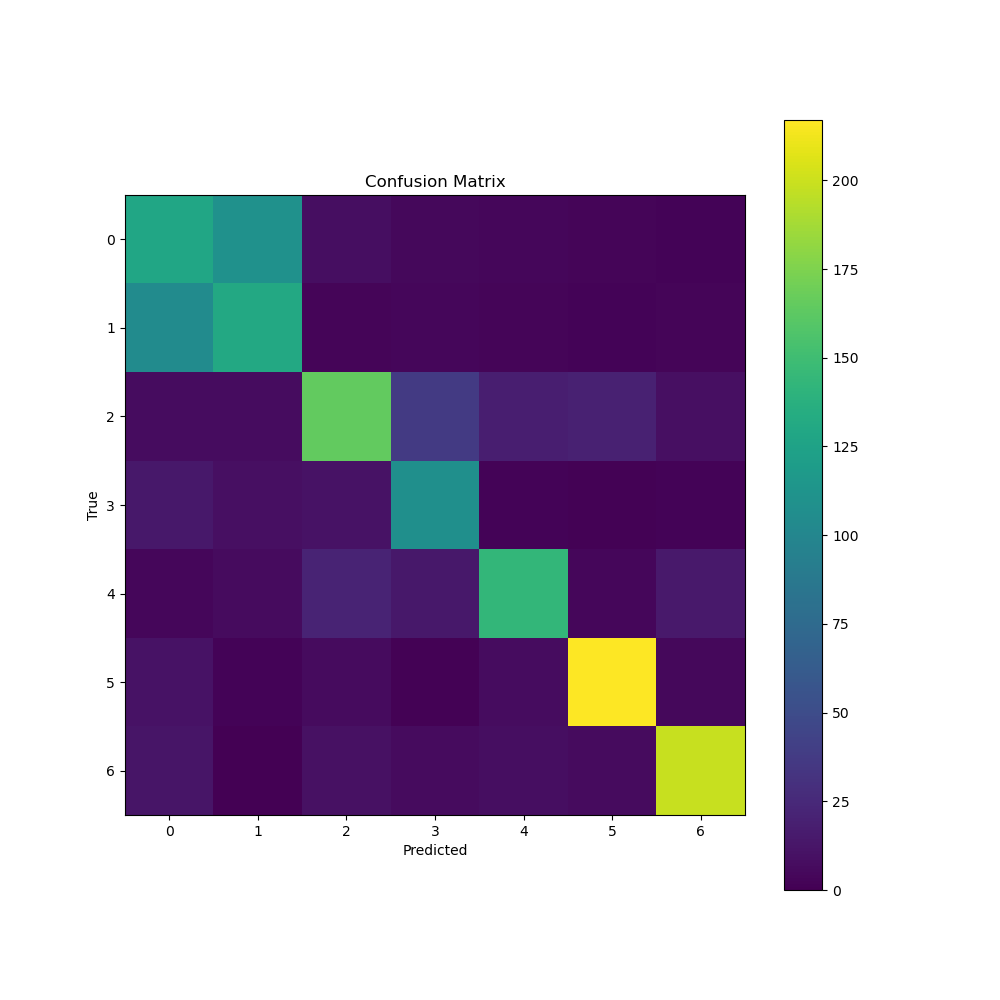
\includegraphics[width=\textwidth]{./pic/confusion_matrix_1641.png}
        \caption{Train Confusion Matrix}
        \label{fig:confusion_matrix_train}
    \end{subfigure}
    \hfill % This command adds space between the subfigures
    \begin{subfigure}{0.45\textwidth}
        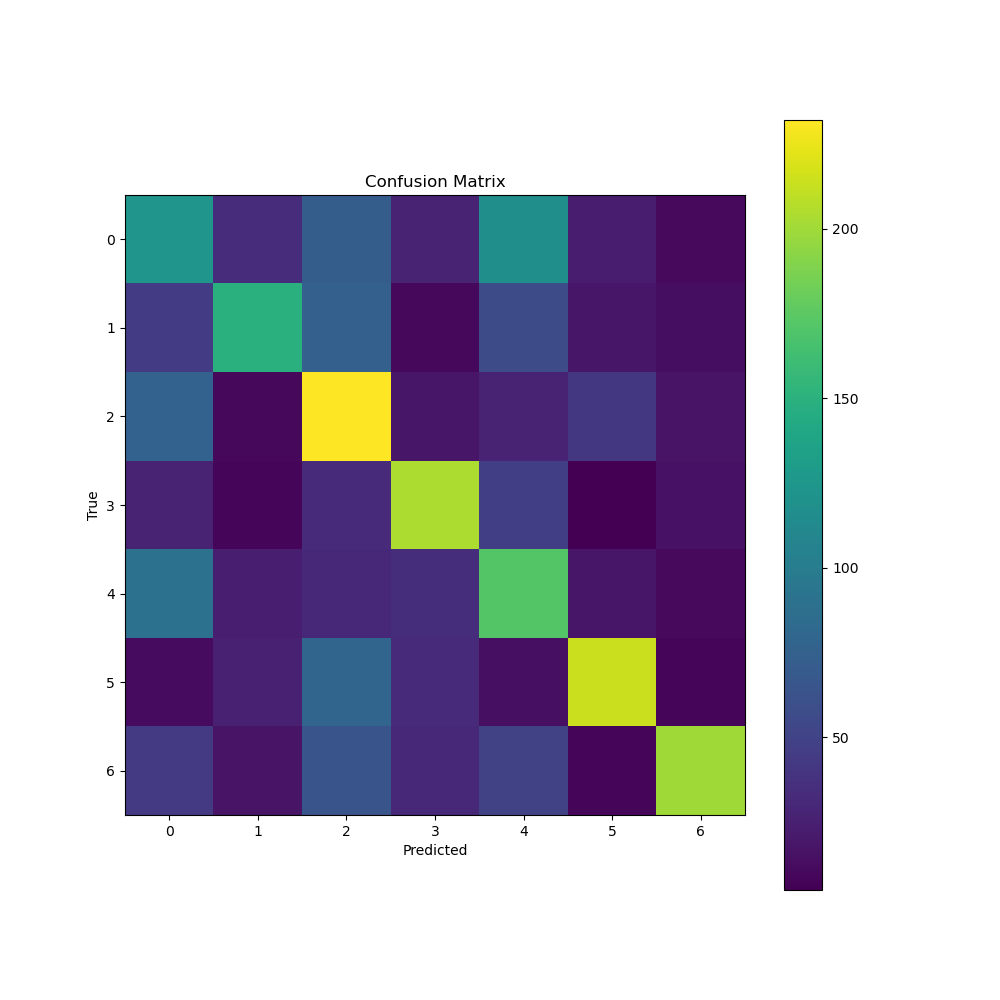
\includegraphics[width=\textwidth]{./pic/confusion_matrix_2723.png}
        \caption{Test Confusion Matrix}
        \label{fig:confusion_matrix_test}
    \end{subfigure}
    \caption{Confusion Matrix}
\end{figure}

\subsubsection*{[Q14]}

The figure \ref{fig:misclassified} shows the misclassified images.
These figures show that the model may not be able to classify those images with complex backgrounds and multiple objects very well.
Also, they may be too vague, concise and unconventional.

Moreover, most of these misclassified data are coming from those type-animal pairs that have less training samples, such as cartoon-dog.

\begin{center}
    \noindent 
    \begin{minipage}{0.142\textwidth}
        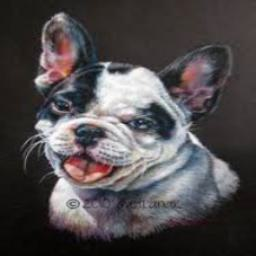
\includegraphics[width=\linewidth]{./pic/misclassified_r0_p2_2723.jpg}
        dog-giraffe
    \end{minipage}%
    \begin{minipage}{0.142\textwidth}
        
\includegraphics[width=\linewidth]{./pic/misclassified_r0_p3_2723.jpg}
        dog-guitar
    \end{minipage}%
    \begin{minipage}{0.142\textwidth}
        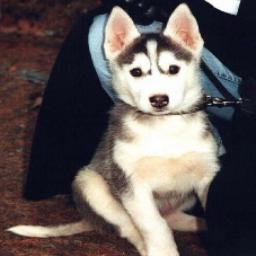
\includegraphics[width=\linewidth]{./pic/misclassified_r0_p6_2723.jpg}
        dog-person
    \end{minipage}%
    \begin{minipage}{0.142\textwidth}
        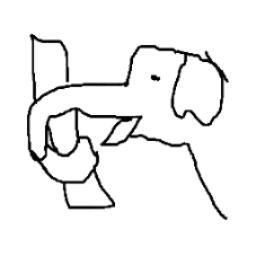
\includegraphics[width=\linewidth]{./pic/misclassified_r1_p0_2723.jpg}
        elephant-dog
    \end{minipage}%
    \begin{minipage}{0.142\textwidth}
        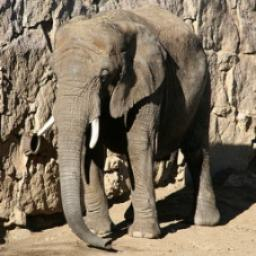
\includegraphics[width=\linewidth]{./pic/misclassified_r1_p2_2723.jpg}
        elephant-giraffe
    \end{minipage}%
    \begin{minipage}{0.142\textwidth}
        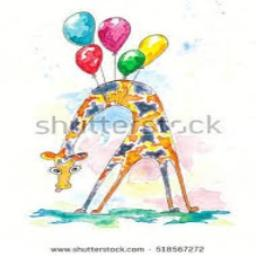
\includegraphics[width=\linewidth]{./pic/misclassified_r2_p3_2723.jpg}
        giraffe-guitar
    \end{minipage}%
    \begin{minipage}{0.142\textwidth}
        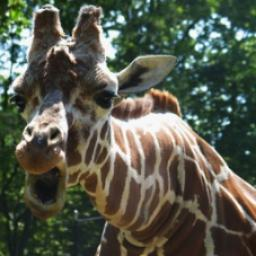
\includegraphics[width=\linewidth]{./pic/misclassified_r2_p4_2723.jpg}
        giraffe-horse
    \end{minipage}%

    % 新的一行
    \noindent
    \begin{minipage}{0.142\textwidth}
        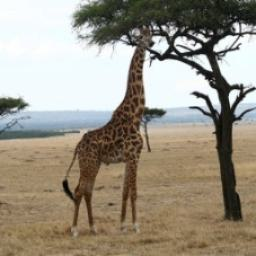
\includegraphics[width=\linewidth]{./pic/misclassified_r2_p5_2723.jpg}
        giraffe-house
    \end{minipage}%
    \begin{minipage}{0.142\textwidth}
        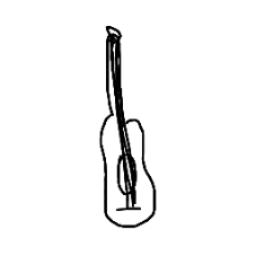
\includegraphics[width=\linewidth]{./pic/misclassified_r3_p0_2723.jpg}
        guitar-dog
    \end{minipage}%
    \begin{minipage}{0.142\textwidth}
        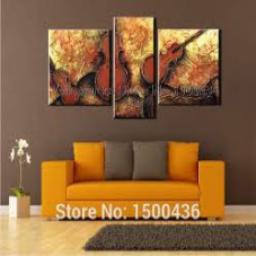
\includegraphics[width=\linewidth]{./pic/misclassified_r3_p4_2723.jpg}
        guitar-horse
    \end{minipage}%
    \begin{minipage}{0.142\textwidth}
        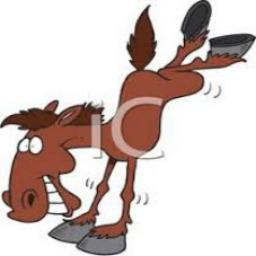
\includegraphics[width=\linewidth]{./pic/misclassified_r4_p3_2723.jpg}
        horse-guitar
    \end{minipage}%
    \begin{minipage}{0.142\textwidth}
        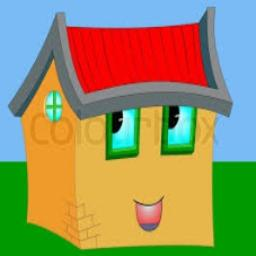
\includegraphics[width=\linewidth]{./pic/misclassified_r5_p4_2723.jpg}
        house-horse
    \end{minipage}%
    \begin{minipage}{0.142\textwidth}
        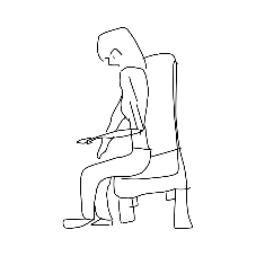
\includegraphics[width=\linewidth]{./pic/misclassified_r6_p0_2723.jpg}
        person-dog
    \end{minipage}%
    \begin{minipage}{0.142\textwidth}
        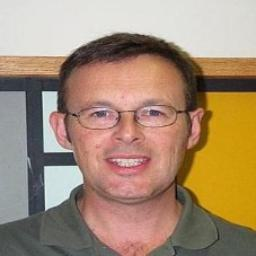
\includegraphics[width=\linewidth]{./pic/misclassified_r6_p4_2723.jpg}
        person-horse
    \end{minipage}%

    \captionof{figure}{Misclassified Images (the label below is [true label]-[wrong label])}
    \label{fig:misclassified}
\end{center}

\subsection*{7.6 Data Augmentation by Style Transfer}

\subsubsection*{[Q15]}

In figure \ref{fig:label_style}, we can see the example of images with labels and styles.

\begin{figure}[htp]
    \centering
    \begin{minipage}{0.14285714285714285\linewidth}
        \includegraphics[width=\linewidth]{./classify/derived-files/dog_art\_painting_0.jpg}
        {dog-art\_painting}
    \end{minipage}%%
    \begin{minipage}{0.14285714285714285\linewidth}
        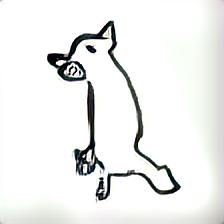
\includegraphics[width=\linewidth]{./classify/derived-files/dog_cartoon_0.jpg}
        {dog-cartoon}
    \end{minipage}%%
    \begin{minipage}{0.14285714285714285\linewidth}
        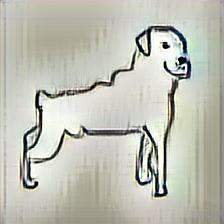
\includegraphics[width=\linewidth]{./classify/derived-files/dog_photo_0.jpg}
        {dog-photo}
    \end{minipage}%%
    \begin{minipage}{0.14285714285714285\linewidth}
        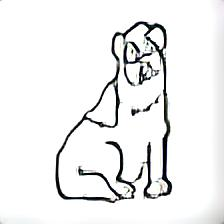
\includegraphics[width=\linewidth]{./classify/derived-files/dog_sketch_0.jpg}
        {dog-sketch}
    \end{minipage}%%
    \begin{minipage}{0.14285714285714285\linewidth}
        \includegraphics[width=\linewidth]{./classify/derived-files/elephant_art\_painting_0.jpg}
        {elephant-art\_painting}
    \end{minipage}%%
    \begin{minipage}{0.14285714285714285\linewidth}
        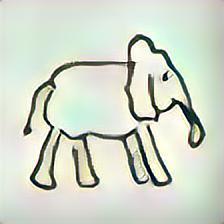
\includegraphics[width=\linewidth]{./classify/derived-files/elephant_cartoon_0.jpg}
        {elephant-cartoon}
    \end{minipage}%%
    \begin{minipage}{0.14285714285714285\linewidth}
        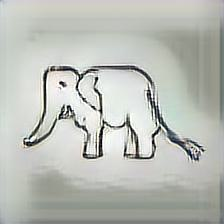
\includegraphics[width=\linewidth]{./classify/derived-files/elephant_photo_0.jpg}
        {elephant-photo}
    \end{minipage}%

    \begin{minipage}{0.14285714285714285\linewidth}
        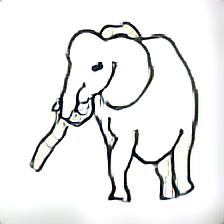
\includegraphics[width=\linewidth]{./classify/derived-files/elephant_sketch_0.jpg}
        {elephant-sketch}
    \end{minipage}%%
    \begin{minipage}{0.14285714285714285\linewidth}
        \includegraphics[width=\linewidth]{./classify/derived-files/giraffe_art\_painting_0.jpg}
        {giraffe-art\_painting}
    \end{minipage}%%
    \begin{minipage}{0.14285714285714285\linewidth}
        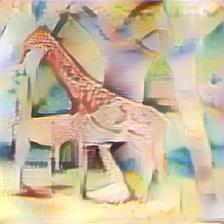
\includegraphics[width=\linewidth]{./classify/derived-files/giraffe_cartoon_0.jpg}
        {giraffe-cartoon}
    \end{minipage}%%
    \begin{minipage}{0.14285714285714285\linewidth}
        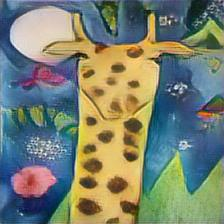
\includegraphics[width=\linewidth]{./classify/derived-files/giraffe_photo_0.jpg}
        {giraffe-photo}
    \end{minipage}%%
    \begin{minipage}{0.14285714285714285\linewidth}
        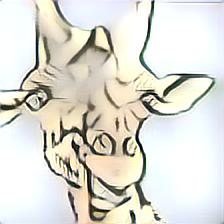
\includegraphics[width=\linewidth]{./classify/derived-files/giraffe_sketch_0.jpg}
        {giraffe-sketch}
    \end{minipage}%%
    \begin{minipage}{0.14285714285714285\linewidth}
        \includegraphics[width=\linewidth]{./classify/derived-files/guitar_art\_painting_0.jpg}
        {guitar-art\_painting}
    \end{minipage}%%
    \begin{minipage}{0.14285714285714285\linewidth}
        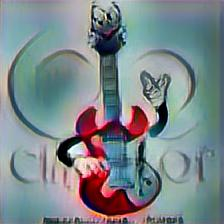
\includegraphics[width=\linewidth]{./classify/derived-files/guitar_cartoon_0.jpg}
        {guitar-cartoon}
    \end{minipage}%

    \begin{minipage}{0.14285714285714285\linewidth}
        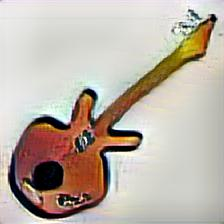
\includegraphics[width=\linewidth]{./classify/derived-files/guitar_photo_0.jpg}
        {guitar-photo}
    \end{minipage}%%
    \begin{minipage}{0.14285714285714285\linewidth}
        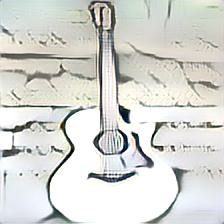
\includegraphics[width=\linewidth]{./classify/derived-files/guitar_sketch_0.jpg}
        {guitar-sketch}
    \end{minipage}%%
    \begin{minipage}{0.14285714285714285\linewidth}
        \includegraphics[width=\linewidth]{./classify/derived-files/horse_art\_painting_0.jpg}
        {horse-art\_painting}
    \end{minipage}%%
    \begin{minipage}{0.14285714285714285\linewidth}
        \includegraphics[width=\linewidth]{./classify/derived-files/horse_cartoon_0.jpg}
        {horse-cartoon}
    \end{minipage}%%
    \begin{minipage}{0.14285714285714285\linewidth}
        \includegraphics[width=\linewidth]{./classify/derived-files/horse_photo_0.jpg}
        {horse-photo}
    \end{minipage}%%
    \begin{minipage}{0.14285714285714285\linewidth}
        \includegraphics[width=\linewidth]{./classify/derived-files/horse_sketch_0.jpg}
        {horse-sketch}
    \end{minipage}%%
    \begin{minipage}{0.14285714285714285\linewidth}
        \includegraphics[width=\linewidth]{./classify/derived-files/house_art\_painting_0.jpg}
        {house-art\_painting}
    \end{minipage}%

    \begin{minipage}{0.14285714285714285\linewidth}
        \includegraphics[width=\linewidth]{./classify/derived-files/house_cartoon_0.jpg}
        {house-cartoon}
    \end{minipage}%%
    \begin{minipage}{0.14285714285714285\linewidth}
        \includegraphics[width=\linewidth]{./classify/derived-files/house_photo_0.jpg}
        {house-photo}
    \end{minipage}%%
    \begin{minipage}{0.14285714285714285\linewidth}
        \includegraphics[width=\linewidth]{./classify/derived-files/house_sketch_0.jpg}
        {house-sketch}
    \end{minipage}%%
    \begin{minipage}{0.14285714285714285\linewidth}
        \includegraphics[width=\linewidth]{./classify/derived-files/person_art\_painting_0.jpg}
        {person-art\_painting}
    \end{minipage}%%
    \begin{minipage}{0.14285714285714285\linewidth}
        \includegraphics[width=\linewidth]{./classify/derived-files/person_cartoon_0.jpg}
        {person-cartoon}
    \end{minipage}%%
    \begin{minipage}{0.14285714285714285\linewidth}
        \includegraphics[width=\linewidth]{./classify/derived-files/person_photo_0.jpg}
        {person-photo}
    \end{minipage}%%
    \begin{minipage}{0.14285714285714285\linewidth}
        \includegraphics[width=\linewidth]{./classify/derived-files/person_sketch_0.jpg}
        {person-sketch}
    \end{minipage}%


\caption{Example of images with labels and styles.}
\label{fig:label_style}
\end{figure}

\subsection*{7.7 Retraining with Augmented Dataset}

\subsubsection*{[Q16]}

After 300 epochs, the cross-entropy loss is 0.874.

\subsubsection*{[Q17]}
The accuracy of training dataset is 0.670, and the accuracy of testing dataset is 0.257.

The confusion matrix is shown in the table \ref{tab:confusion_matrix_train_aug} and table \ref{tab:confusion_matrix_test_aug}.

Also, I visualize the confusion matrix in the figure \ref{fig:confusion_matrix_train_aug} and figure \ref{fig:confusion_matrix_test_aug}.

\begin{center}
    \textbf{Confusion Matrix for Train}
    
    \begin{tabular}{c|ccccccc}
    \toprule
    & \multicolumn{7}{c}{Predicted Labels} \\
    \cmidrule(lr){2-8}
    True Labels & dog & elephant & giraffe & guitar & horse & house & person \\
    \midrule
    dog & 340 & 49 & 18 & 14 & 17 & 5 & 10 \\
    elephant & 223 & 143 & 20 & 21 & 13 & 14 & 19 \\
    giraffe & 19 & 14 & 319 & 33 & 25 & 14 & 36 \\
    guitar & 33 & 22 & 42 & 209 & 20 & 8 & 13 \\
    horse & 14 & 20 & 33 & 21 & 283 & 15 & 21 \\
    house & 18 & 14 & 16 & 4 & 11 & 364 & 17 \\
    person & 13 & 11 & 20 & 14 & 7 & 22 & 357 \\
    \bottomrule
    \end{tabular}
    \captionof{table}{Confusion matrix for the training dataset.}
    \label{tab:confusion_matrix_train_aug}
\end{center}

\begin{center}
    \textbf{Confusion Matrix for Test}
    
    \begin{tabular}{c|ccccccc}
    \toprule
    & \multicolumn{7}{c}{Predicted Labels} \\
    \cmidrule(lr){2-8}
    True Labels & dog & elephant & giraffe & guitar & horse & house & person \\
    \midrule
    dog & 123 & 18 & 58 & 64 & 54 & 44 & 45 \\
    elephant & 124 & 45 & 44 & 47 & 38 & 33 & 38 \\
    giraffe & 104 & 19 & 126 & 75 & 40 & 36 & 24 \\
    guitar & 96 & 32 & 43 & 75 & 43 & 25 & 26 \\
    horse & 97 & 36 & 41 & 42 & 103 & 37 & 26 \\
    house & 67 & 49 & 51 & 30 & 44 & 121 & 24 \\
    person & 54 & 87 & 48 & 38 & 57 & 23 & 106 \\
    \bottomrule
    \end{tabular}
    \captionof{table}{Confusion matrix for the testing dataset.}
    \label{tab:confusion_matrix_test_aug}
\end{center}

        
    
\begin{figure}[h!]
    \centering
    % First row of subfigures
    \begin{subfigure}{0.45\textwidth}
        \includegraphics[width=\textwidth]{./pic/confusion_matrix_3041.png}
        \caption{Train Confusion Matrix}
        \label{fig:confusion_matrix_train_aug}
    \end{subfigure}
    \hfill % This command adds space between the subfigures
    \begin{subfigure}{0.45\textwidth}
        \includegraphics[width=\textwidth]{./pic/confusion_matrix_2723_1.png}
        \caption{Test Confusion Matrix}
        \label{fig:confusion_matrix_test_aug}
    \end{subfigure}
    \caption{Confusion Matrix}
\end{figure}

Comparing the confusion matrix of the original model and the model with augmented dataset, 
we can see that the model with augmented dataset has a little bit better performance.

\subsubsection*{[Q18]}
This result may be caused by the fact that the augmented dataset has more samples and more styles,
which can help the model learn more features and be more robust.

\end{document}
